\documentclass{llncs}

\usepackage{makeidx}  % allows for indexgeneration

\usepackage{graphics, graphicx, xcolor}

%\usepackage{times}

\newcommand{\authcmt}[2]{\textcolor{#1}{#2}}
\newcommand{\yuncong}[1]{\authcmt{red}{[YC: #1]}}
\newcommand{\yoav}[1]{\authcmt{blue}{[YF: #1]}}

\begin{document}
%
%\mainmatter              % start of the contributions
%
\title{Robust Landmark Detection for Mouse Brain Section Images}
%
\titlerunning{Robust Region Landmark Detection}  % abbreviated title (for running head)
%                                     also used for the TOC unless
%                                     \toctitle is used
%
\author{Yuncong Chen \and Yoav Freund}
%
\authorrunning{Yuncong Chen et al.} % abbreviated author list (for running head)
%
%%%% list of authors for the TOC (use if author list has to be modified)
\tocauthor{Yuncong Chen, Yoav Freund}
%
\institute{Department of Computer Science and Engineering, \\University of California, San Diego, La Jolla, CA 92122, USA}




\maketitle              % typeset the title of the contribution

\begin{abstract}

Brightfield and flurescent imaging is of central importance in mouse brain
studies. As automation is improving, a whole brain can be imaged in 
one hour. At the same time, there is an increasing number of
fluorescent markers that can be used to identify neurons with specific
phenotypes. As the number of available images mounts, the manual work
required to analyze these images becomes a major bottleneck and 
automated tools for processing those images become necessary.

In this work we describe the first steps in a project whose goal is to
create a ``digital atlas'' of the brain. A digital atlas in this
context is computer software (and data) that takes as input a stack of
section images and maps those images onto a standarized coordinate
system for the mouse brain. Such mapping is a prerquisite for
automatic quantitative analysis of phenotypical variation. Currently
such mapping is done manually.

The part of the project described here is a semi-supervised learning
system for identifying landmarks in brain slice images. The
identification of such landmarks is based on identifying regions with
distinct texture and the boundaries between these landmarks. Thew
digital atlas will be compiled by comparing different brains and
identifying the consistent landmarks.

\iffalse
Neuronal circuits in the mouse brainstem controls important functions such as breathing and whisking. Studying these circuits has been a center-point of neuroscience, but the difficulties associated with identifying functional cell types and their spatial organization has been a major impediment to the advancement in these studies. We propose a system that automatically constructs atlases marked with important anatomical regions. By defining interesting regions as those with high statistical significance in its neighborhood, our algorithm identifies regions that are both distinct in texture and robust between different sections. Experiments show that the detected regions have high correspondences with labelings provided by experienced anatomists. The results serve as the cornerstone for 3D registration and 3D atlas building.
\fi

\keywords{landmark detection, atlas generation, mouse brain, gabor filter}
\end{abstract}
%

\yoav{Overall, good outline. Next steps are to write an abstract and
  to generate good figures. I would write the text after having the
  figures.}

\section{Introduction}
%

Registering brainstem is hard due to the lack of high contrast edges,
compared to Cerebral Cortex and Cerebellum. One has to rely on
differences in texture.

\yoav{The Allen Reference Atlas is only useful to humans, it is not a
  system that can take a stack and align it to a standard. In
  addition, it has limited details in the brain stem. Partha Mitra
  actually had an interesting suggestion, which is that we get the
  atlas images and annotation and use them to train texture
  detectors.}

Allen Reference Atlas does not have enough details in brainstem.


Not just registration, we want to summarize the regions of interest in the images.


\section{Related Work}

\begin{description}

\item{Point Landmark Detection}

SIFT

\item{Saliency and Objectness Detection}

global rarity scheme

center-surround scheme

\yoav{Is there work that uses notion of statistical significance in
  this context?}

\item{Texture Representation}

gabor filter

textons

\end{description}

\section{Representing Texture using Histograms of Gabor Textons}

Our algorithm starts with representing textures using responses of Gabor filters. Regions are detected based on similar textures. Regions with high contrast are selected. 

  Boundaries that are consistently part of region

We filter the image use Gabor filters.




%\begin{figure}
%\caption{Gabor Filters}
%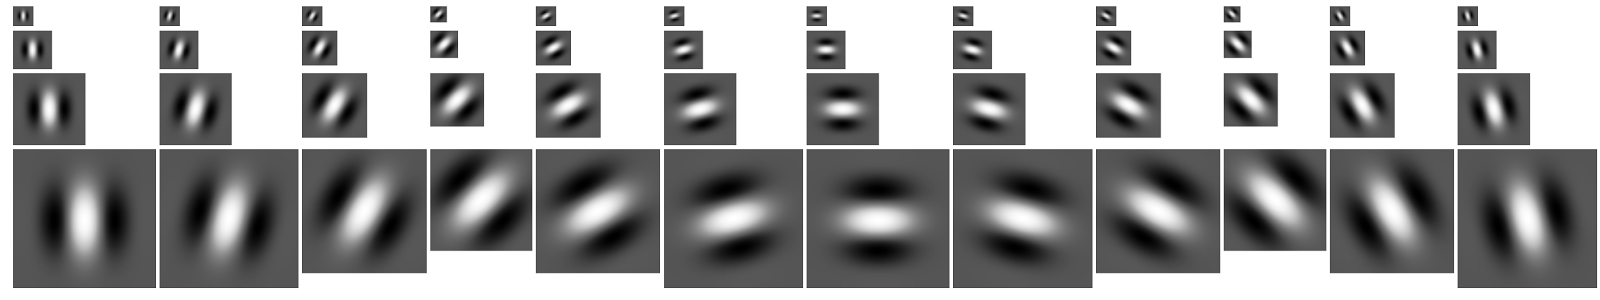
\includegraphics[width=0.5\textwidth]{../figures/gabor}
%\end{figure}


rotation-invariant k-means clustering to form textons.

Over-segment into superpixels.

Describe texture using histogram of textons

\section{Detecting Significant Region Using Center-Surround Contrast}

\yoav{Define the problem of finding regions+textures of high
  statistical significance.}


Brain anatomists usually label section images in terms of nuclei, which are dense groups of gray matter with the same phenotype. For example, Figure 1 shows the facial motor nucleus. Nuclei are typically well localized and are visually salient. In other words, they are constrained regions whose texture is stable within itself but distinct from its surrounds. These characteristics of nuclei allow them to be identified automatically when constructing the atlas, and also make them natural landmarks for registration. In addition to nuclei, fiber tracts are also easily recognizable structures. In particular, the orientation of a tract serves as an important feature of the landmark.

Given the texture descriptors obtained from Gabor textons, we define the saliency of a region in terms of statistical significance computed for texton distributions, as we will elaborate below.
 
\yuncong{We aim to find an algorithm that detects salient regions
define saliency in terms of statistical significance. That is, salient regions should be those whose texton histogram is unlikely to be generated by those of the surrounds.}
 
First, region growing is performed on each superpixel. Starting from a region with one particular superpixel, the greedy procedure considers all superpixels that are neighbors of the current region, and iteratively adds the one whose texton distribution is most similar to the average distribution of the current region. Distance of texton distributions is computed using the Jenson-Shannon divergence, which is a symmetric measure.

Instead of using a pre-determined threshold on the distribution distance between the newly added superpixel and the current region average as the termination criteria, we over-grow the region (until 10\% of the total area) while recording the distances at every iteration, and eventually return the region when the distance is the largest in retrospect. In this way, a region automatically grows to the place where the interior-exterior contrast is the greatest.

We call the region that grows out of a seed superpixel the \textit{expansion cluster} of that superpixel.

The significance of a region can be defined using a similar metric, that is the smallest distribution distance between any neighbor and the current region average. If the distance is the Kullback-Leibler divergence, then via Sanov's theorem, this value can be interpreted as the statistical significance of observing the interior texton histogram given that the closest neighbor's histogram is the true distribution.

\section{Human Supervision}

\yoav{Describe how salient region detection improves efficiency of human labeling.}

\section{Detecting Boundaries by Region Consensus}

\yuncong{Major points for this section: (1) Boundaries are more robust landmarks than regions. (2) Why detect  boundary segments? It is too crude to compute a single saliency value for a region. It is important to characterize saliency in different sides of the region, that is why we associate saliency value with boundary segments, rather than with entire regions. Also often regions are salient relative to each other, in this case using boundary is a more compact representation.}

Because region growing is not perfect, the expansion clusters of superpixels that belong to the same nucleus are often not identical. Figure x shows one such example. In most cases, boundaries are more robust landmarks than areas.

In addition to closed contours, partial boundaries are useful in cases when there is a clear boundary on one side of the nucleus where most clusters agree on, while on the other side no definitive boundary is present.


We aim to identify robust boundary segments that are supported by a large number of clusters. The strategy is to let the clusters vote for their boundaries using their respective significance scores. Superpixels receive high boundary votes if they are at the exterior of many salient clusters.


Instead of letting each superpixel as boundary separately, vote for them as a set.

Each region votes according to their saliency scores.

Each boundary is described by a tuple that consists of four elements:

1. x-y positions of every superpixel on the boundary

2. centroid of the expansion cluster inside the boundary

3. the average texton distribution of interior superpixels

4. a list of texton distributions of exterior superpixels (more precisely, the closest layer of superpixels on the outside of the boundary).

\section{Matching Boundaries from Different Sections}

distance = interior + exterior + shape + location 
\\

Distance between boundaries are defined as a weighted combination of:

1. Jenson-Shannon divergence between interior distributions

2. symmetric Hausdorff distances between the two sets of exterior distributions. That is, the maximum among the distances between each distribution and its closest distribution from the other set. Here the distance is the Jenson-Shannon divergence.

3. shape dissimilarity: total chi2-distances of shape context descriptors after correspondences are identified for superpixels on two boundaries using dynamic programming. (This is essentially the Shape Distance in Section 5.1 of Belongie's paper)

4. spatial distance: Euclidean distance between cluster centroids
\\

Boundaries are detected from two sections and their pairwise distances are computed. A pair of boundaries are matched if they are the closest boundary of each other.

\section{Experiments}

\subsection{comparison with human labelings}

Shows the results of our algorithm is comparable to human labeling.

show results for RS141. (Do we need to do more than one stacks here? I think one stack already shows enough variations. A coronal stack would be good, but we don't have any now).

\subsection{robustness of matching}

Shows that matchings are robust to distortion and shape change.
Also shows that our distance measure is a sensible one: each of the four terms is important. We show this by changing the term weightings, and then compare matching results.

\section{Future Work}

use detected landmarks for registration

Learn dictionary using deep neural networks, ICA, ...



%
% ---- Bibliography ----
%
\begin{thebibliography}{5}
%
\bibitem {clar:eke}
Clarke, F., Ekeland, I.:
Nonlinear oscillations and
boundary-value problems for Hamiltonian systems.
Arch. Rat. Mech. Anal. 78, 315--333 (1982)

\end{thebibliography}


\end{document}
